
\chapter{O que é Machine Learning?}

Machine Learning, ou aprendizado de máquina, é uma área da Inteligência Artificial que permite que sistemas computacionais aprendam a identificar padrões, analisar informações e realizar previsões a partir de dados, sem que todas as suas regras de funcionamento precisem ser programadas manualmente. Em vez de receber instruções específicas para cada situação, o sistema utiliza exemplos e informações disponíveis para identificar relações e desenvolver modelos capazes de realizar determinadas tarefas.

Na prática, isso significa que um sistema de Machine Learning pode analisar um grande conjunto de informações, identificar características em comum e utilizar esses conhecimentos para tomar decisões ou realizar previsões sobre novos dados. Por exemplo, ao analisar milhares de mensagens classificadas como spam ou legítimas, um algoritmo pode aprender a reconhecer características comuns em mensagens indesejadas e utilizar esse conhecimento para classificar novos e-mails automaticamente.

Dessa forma, o aprendizado de máquina possibilita que computadores executem tarefas que normalmente exigiriam análise humana, como reconhecimento de imagens, identificação de padrões, previsão de resultados, classificação de informações e personalização de serviços. Seu funcionamento está diretamente relacionado à quantidade, qualidade e relevância dos dados utilizados no processo de treinamento, uma vez que essas informações influenciam a capacidade do modelo de identificar padrões e produzir resultados adequados \cite{googlecloudML, ibmML}.

\chapter{Como funciona o Machine Learning?}

O funcionamento do Machine Learning envolve, principalmente, a coleta de dados, seu processamento, o treinamento de um modelo e a utilização desse modelo para realizar previsões ou classificações. Inicialmente, são reunidas informações relacionadas ao problema que se deseja solucionar. Esses dados podem ser provenientes de diferentes fontes, como registros de compras, imagens, textos, sensores, históricos de utilização de sistemas, informações financeiras ou dados de localização.

Após a coleta, os dados passam por um processo de preparação, no qual podem ser organizados, tratados e corrigidos para reduzir inconsistências e permitir que o algoritmo consiga utilizá-los adequadamente. Em seguida, um algoritmo de aprendizado de máquina analisa essas informações em busca de padrões, relações entre variáveis e características relevantes para a tarefa proposta.

Durante o treinamento, o modelo ajusta seus parâmetros com base nos dados disponíveis, buscando melhorar seus resultados. Dependendo da abordagem utilizada, esse processo pode ocorrer por meio da comparação entre previsões e respostas conhecidas, da identificação de agrupamentos ou da avaliação das consequências de determinadas ações. Quando o treinamento é concluído, o modelo pode receber novos dados e produzir resultados com base nos padrões que aprendeu anteriormente \cite{ibmML, awsML}.

Existem diferentes formas de treinamento de modelos de Machine Learning, sendo algumas das principais:

\section{Aprendizado supervisionado}

O aprendizado supervisionado utiliza conjuntos de dados que possuem exemplos acompanhados de respostas previamente conhecidas. Durante o treinamento, o algoritmo analisa as informações de entrada e compara suas previsões com os resultados esperados, ajustando seu funcionamento para reduzir os erros.

Essa abordagem é utilizada principalmente em problemas de classificação e previsão. Um exemplo seria um sistema que analisa informações de clientes, como histórico de pagamentos e renda, para estimar a probabilidade de inadimplência. Outro exemplo é o reconhecimento de imagens, no qual o modelo aprende a identificar objetos a partir de imagens previamente classificadas \cite{googleSupervised, ibmML}.

\section{Aprendizado não supervisionado}

O aprendizado não supervisionado utiliza dados que não possuem respostas previamente definidas. Nesse caso, o algoritmo procura identificar padrões, semelhanças, agrupamentos e relações existentes nas informações analisadas.

Uma aplicação dessa abordagem ocorre na segmentação de clientes. Uma empresa pode utilizar dados de compras, frequência de consumo e preferências para identificar grupos de consumidores com comportamentos semelhantes, permitindo desenvolver estratégias de marketing mais direcionadas. Também pode ser utilizado para detectar comportamentos incomuns, que eventualmente indiquem fraudes ou anomalias \cite{googleUnsupervised, ibmML}.

\section{Aprendizado por reforço}

O aprendizado por reforço é uma abordagem na qual um sistema aprende a tomar decisões por meio da interação com um ambiente. A cada ação realizada, o sistema recebe algum tipo de retorno, que pode representar uma recompensa ou uma penalidade, de acordo com o resultado obtido.

Com base nesses retornos, o modelo busca identificar quais ações são mais adequadas para alcançar determinado objetivo ao longo do tempo. Essa abordagem pode ser utilizada em robótica, jogos digitais, sistemas de otimização e situações que envolvam decisões sequenciais, nas quais uma ação pode influenciar os resultados futuros \cite{ibmML, awsML}.

\chapter{Onde o Machine Learning é utilizado?}

O Machine Learning está presente em diferentes setores da sociedade, sendo utilizado para automatizar processos, melhorar serviços, analisar grandes volumes de informações e auxiliar na tomada de decisões. Muitas de suas aplicações estão incorporadas a ferramentas utilizadas diariamente, mesmo quando os usuários não percebem diretamente a presença dessa tecnologia.

\section{Sistemas de recomendação da Netflix}

Uma aplicação bastante conhecida do Machine Learning está nos sistemas de recomendação utilizados por plataformas de streaming, como a Netflix. A plataforma utiliza algoritmos para analisar diferentes informações relacionadas ao comportamento dos usuários, como conteúdos assistidos, interações, preferências, pesquisas realizadas e características dos filmes e séries disponíveis.

Com base nesses dados, os modelos identificam padrões de interesse e estimam quais conteúdos podem ser mais relevantes para cada usuário. Dessa maneira, as recomendações apresentadas na página inicial podem variar de acordo com os hábitos e preferências individuais, contribuindo para que cada pessoa encontre conteúdos de seu interesse com maior facilidade.

A Netflix utiliza diferentes modelos e técnicas de aprendizado de máquina para personalizar recomendações, organizar conteúdos e aprimorar a experiência de seus assinantes. Esse tipo de aplicação demonstra como o Machine Learning pode ser utilizado para personalização de serviços em larga escala \cite{netflixResearch, netflixRecommender}.

\section{Detecção de spam e segurança no Gmail}

Outra aplicação cotidiana do Machine Learning pode ser observada no Gmail, serviço de e-mail da Google. A plataforma utiliza modelos de aprendizado de máquina para identificar mensagens potencialmente indesejadas, como spam, tentativas de phishing e e-mails maliciosos.

Para realizar essa identificação, os sistemas podem analisar diversas características das mensagens, incluindo o conteúdo textual, informações sobre remetentes, padrões de envio, links e outros sinais associados a comportamentos suspeitos. A partir dessas informações, os modelos estimam a probabilidade de uma mensagem representar uma ameaça ou ser indesejada.

Essa aplicação é importante porque a quantidade de mensagens recebidas diariamente torna inviável uma análise manual de todas elas. O Machine Learning permite que esse processo seja realizado automaticamente, contribuindo para a segurança dos usuários e reduzindo a exposição a golpes e conteúdos maliciosos. A Google utiliza modelos de aprendizado de máquina em conjunto com outras técnicas de segurança para aprimorar a identificação de mensagens suspeitas \cite{googleGmailML, googleSpamTensorflow}.

\section{Previsões e análise de trânsito no Google Maps}

O Machine Learning também é utilizado em serviços de navegação e mobilidade, como o Google Maps. A ferramenta utiliza dados relacionados ao trânsito para estimar condições das vias, prever congestionamentos e auxiliar na escolha de rotas.

Essas análises podem considerar informações como velocidade dos veículos, histórico de circulação, condições atuais das estradas, localização e outros dados relacionados ao deslocamento. A partir da identificação de padrões, os sistemas conseguem estimar possíveis condições futuras do trânsito e fornecer informações que auxiliam os usuários a planejar suas viagens.

Com isso, o serviço pode oferecer estimativas de tempo de deslocamento, identificar trajetos alternativos e auxiliar na tomada de decisões durante uma viagem. Essa aplicação demonstra como o aprendizado de máquina pode utilizar grandes volumes de dados continuamente atualizados para gerar previsões úteis em situações reais \cite{googleAIMaps}.


\chapter{Quais são os benefícios?}
O Machine Learning (ML) transforma grandes volumes de dados brutos em padrões acionáveis, ampliando a capacidade analítica e operacional de empresas, governos e da sociedade. Em vez de depender exclusivamente de regras programadas manualmente, os modelos aprendem relações estatísticas e ajustam seu desempenho conforme recebem novos dados.

\begin{itemize}
	\item \textbf{Automação inteligente de tarefas complexas e repetitivas:} sistemas de ML assumem atividades rotineiras de triagem, classificação e processamento de dados com alta velocidade e consistência, liberando equipes humanas para análises estratégicas e criativas.
	
	\item \textbf{Apoio à tomada de decisão baseada em evidências:} ao cruzar milhares ou milhões de variáveis, modelos preditivos ajudam gestores, médicos e formuladores de políticas públicas a antecipar cenários, avaliar riscos e alocar recursos com mais precisão.
	
	\item \textbf{Personalização em larga escala:} plataformas digitais, serviços financeiros e sistemas educacionais conseguem adaptar recomendações, ofertas e trilhas de aprendizagem ao perfil e ao ritmo de cada usuário, aumentando a relevância e a acessibilidade dos conteúdos.
	
	\item \textbf{Detecção precoce de anomalias e prevenção de perdas:} no setor financeiro, na indústria e na cibersegurança, algoritmos de ML identificam desvios sutis em tempo real, como transações atípicas em cartões, falhas iminentes em máquinas industriais ou intrusões em redes, antes que o prejuízo se consolide.
	
	\item \textbf{Avanço científico e impacto social:} na saúde, na agricultura e no meio ambiente, o ML acelera a análise de exames, a previsão de safras e o monitoramento de padrões climáticos ou de biodiversidade, ampliando a eficiência de serviços essenciais.
\end{itemize}

\begin{figure}[H]
	\centering
	\caption{Top benefícios de machine learning}
	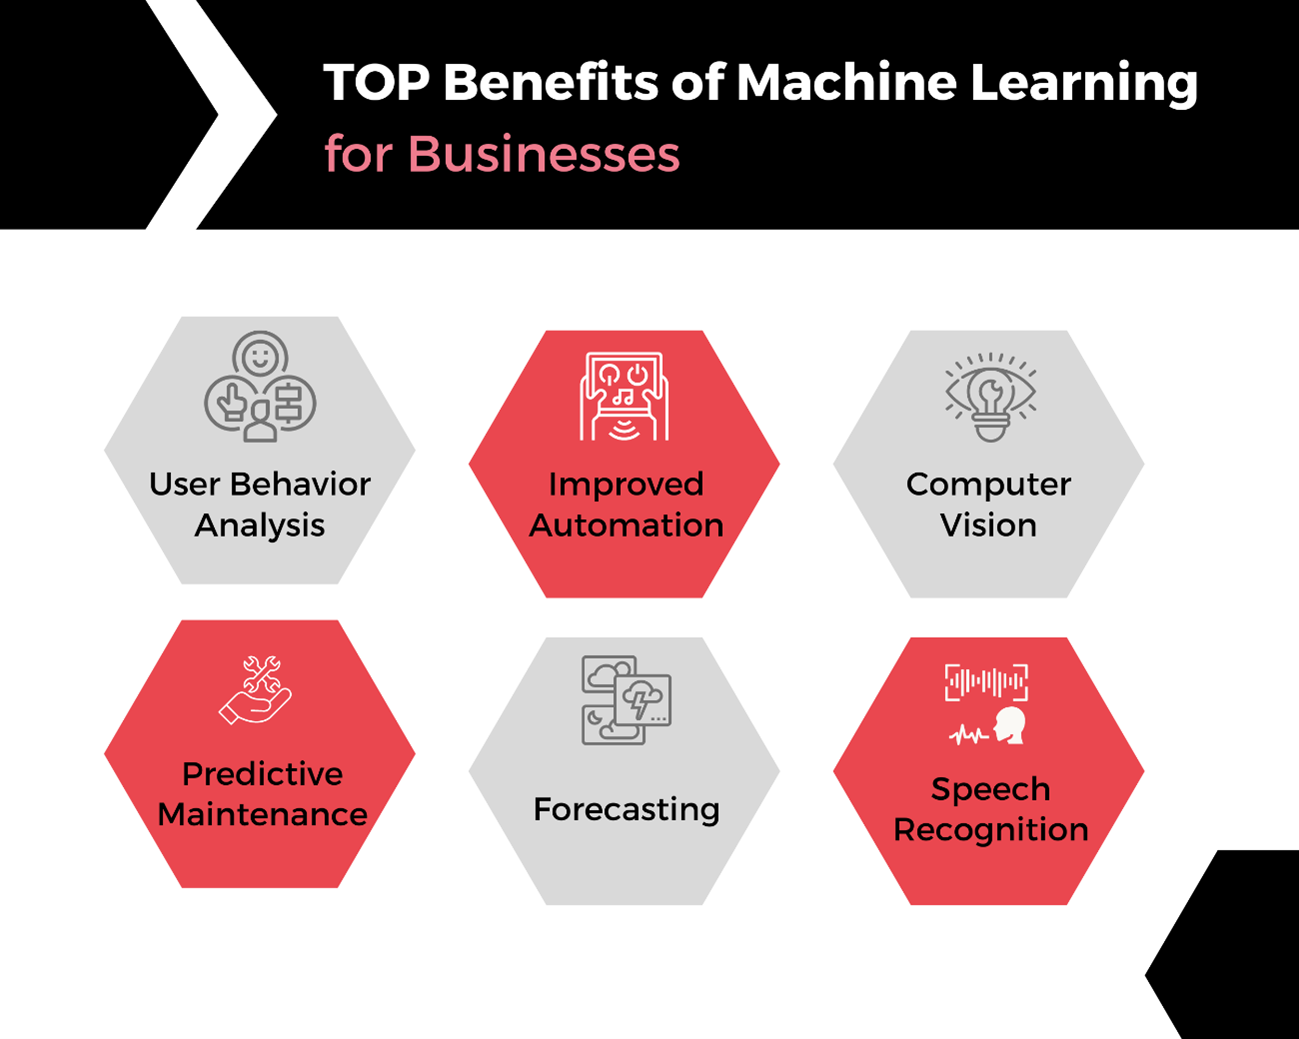
\includegraphics[scale=1]{images/iabenfef.png}
	\fonte{\cite{img1}}
\end{figure}

\chapter{Quais são as limitações ou riscos?}
Apesar do alto potencial, o uso de Machine Learning envolve desafios técnicos, éticos, jurídicos e operacionais que exigem governança rigorosa.

\begin{itemize}
	\item \textbf{Viés algorítmico e discriminação:} modelos treinados com dados históricos que refletem desigualdades sociais ou falhas humanas podem reproduzir e até amplificar preconceitos em áreas sensíveis, como concessão de crédito, recrutamento ou segurança pública.
	
	\item \textbf{Falta de explicabilidade (``caixa-preta''):} muitos modelos avançados atingem alta precisão estatística, mas têm decisões difíceis de interpretar de forma transparente. Isso complica auditorias, responsabilização legal e o direito de contestação de decisões automatizadas (previsto, por exemplo, no artigo 20 da LGPD no Brasil).
	
	\item \textbf{Privacidade, proteção de dados e propriedade intelectual:} o treinamento e a operação de sistemas de ML dependem de grandes bases de dados, o que eleva riscos de exposição indevida de informações pessoais, uso não autorizado de dados ou disputas sobre direitos autorais.
	
	\item \textbf{Dependência de dados de qualidade e \textit{data drift}:} se os dados de entrada forem incompletos, desatualizados ou ruidosos, o modelo errará sistematicamente (``lixo entra, lixo sai''). Além disso, quando o comportamento do mundo real muda ao longo do tempo (\textit{data drift}), modelos estáticos perdem precisão sem retreinamento contínuo.
	
	\item \textbf{Desigualdade de acesso e sobrecarga cognitiva:} a adoção avançada exige infraestrutura computacional, conectividade e qualificação técnica nem sempre disponíveis de forma igualitária entre regiões, escolas ou empresas. Na educação e no trabalho, o uso acrítico também pode gerar dependência tecnológica e reduzir o esforço de reflexão crítica.
\end{itemize}


\begin{figure}[H]
	\centering
	\caption{Vantagens e desvantagens do Machine Learning}
	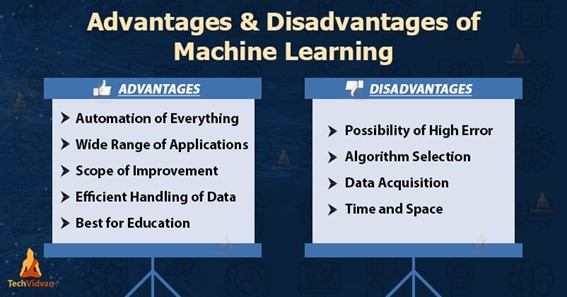
\includegraphics[scale=1]{images/vantagens.jpg}
	\fonte{\cite{img2}}
\end{figure}

\chapter{Qual é o futuro dessa tecnologia?} 


Nos próximos anos, o Machine Learning tende a deixar de ser apenas um recurso isolado de análise estatística para se tornar uma \textbf{camada transversal de infraestrutura} em praticamente todos os setores. 

\begin{itemize}
	\item \textbf{Transformação --- e não extinção simples --- do mercado de trabalho:} relatórios como o \textit{Future of Jobs Report} do Fórum Econômico Mundial indicam que a automação desloca tarefas repetitivas e previsíveis, mas também cria novas funções e amplia a produtividade de quem sabe trabalhar em conjunto com sistemas inteligentes. Em vez de apenas ``substituir profissões'', o ML redesenha tarefas dentro das carreiras.
	
	\item \textbf{Valorização de competências híbridas (técnicas + humanas):} ganharão destaque profissionais capazes de formular boas perguntas, validar resultados, atuar com ética e combinar domínio de dados/ferramentas de IA com pensamento crítico, criatividade, comunicação, liderança e resolução de problemas complexos.
	
	\item \textbf{Modelos mais eficientes, multimodais e supervisionados:} a tendência aponta para sistemas que combinam diferentes tipos de dados (texto, imagem, áudio, sensores), operam com maior eficiência energética e atuam como copilotos ou agentes sob supervisão humana.
\end{itemize}

\begin{table}[htb]
	\centering
	\caption{Oportunidades e desafios do Machine Learning}
	\label{tab:oportunidades_desafios_ml}
	\begin{tabular}{|p{3.2cm}|p{4.2cm}|p{4.2cm}|}
		\hline
		\textbf{Dimensão} & \textbf{Oportunidade / Tendência} & \textbf{Desafio a Superar} \\ \hline
		
		\textbf{Produtividade e processos} & 
		Automação de rotinas e análises mais rápidas & 
		Evitar erros silenciosos por falta de validação humana \\ \hline
		
		\textbf{Mercado de trabalho} & 
		Novas funções e valorização de perfis híbridos & 
		Requalificação contínua e redução da exposição de tarefas repetitivas \\ \hline
		
		\textbf{Ética e sociedade} & 
		Serviços mais acessíveis e decisões baseadas em dados & 
		Combater vieses, proteger dados pessoais e garantir transparência \\ \hline
	\end{tabular}
	\fonte{Elaborado pelos autores (2026).}
\end{table}

\chapter{Considerações finais}

O Machine Learning representa uma das principais aplicações da Inteligência Artificial na atualidade, permitindo que sistemas computacionais analisem grandes quantidades de dados, identifiquem padrões e produzam resultados que auxiliam tanto atividades cotidianas quanto processos complexos realizados por empresas e instituições.

Ao longo da pesquisa, foi possível compreender que seu funcionamento está baseado no aprendizado a partir de dados, possibilitando a realização de tarefas como previsões, classificações, identificação de anomalias e personalização de serviços. Aplicações como os sistemas de recomendação da Netflix, os filtros de segurança do Gmail e as previsões de trânsito do Google Maps demonstram que essa tecnologia já está integrada a diversos serviços utilizados diariamente pela sociedade.

Entretanto, apesar de suas vantagens, a utilização do Machine Learning também exige atenção a aspectos como qualidade dos dados, possíveis erros nas previsões, privacidade, discriminação algorítmica e necessidade de supervisão humana. Dessa forma, seus resultados não devem ser considerados automaticamente corretos, sendo importante que os sistemas sejam desenvolvidos, avaliados e utilizados de maneira responsável.

Conclui-se que o Machine Learning possui grande potencial para transformar a maneira como informações são analisadas, decisões são tomadas e serviços são oferecidos. Sua evolução tende a ampliar ainda mais suas aplicações em diferentes áreas, tornando cada vez mais importante o conhecimento sobre seu funcionamento, suas possibilidades e suas limitações.
```